\chapter{Architecture Constraints}

\label{section:Environment}
\begin{longtable}{|l|l|l|}
\hline
\begin{minipage}{0.30\linewidth}\raggedright\vspace{.75ex}{\cellcolor{eTASPurple}\textcolor{white}{\bfseries Tool Name} }\vspace{.75ex}\end{minipage} & \begin{minipage}{0.23\linewidth}\raggedright\vspace{.75ex}{\cellcolor{eTASPurple}\textcolor{white}{\bfseries Version No.} }\vspace{.75ex}\end{minipage} & \begin{minipage}{0.38\linewidth}\raggedright\vspace{.75ex}{\cellcolor{eTASPurple}\textcolor{white}{\bfseries Description} }\vspace{.75ex}\end{minipage}\\
\hline\hline
\endfirsthead
\hline
\begin{minipage}{0.30\linewidth}\raggedright\vspace{.75ex}{\cellcolor{eTASPurple}\textcolor{white}{\bfseries Tool Name} }\vspace{.75ex}\end{minipage} & \begin{minipage}{0.23\linewidth}\raggedright\vspace{.75ex}{\cellcolor{eTASPurple}\textcolor{white}{\bfseries Version No.} }\vspace{.75ex}\end{minipage} & \begin{minipage}{0.38\linewidth}\raggedright\vspace{.75ex}{\cellcolor{eTASPurple}\textcolor{white}{\bfseries Description} }\vspace{.75ex}\end{minipage}\\
\hline\hline
\endhead
\hline
\endfoot
\hline
\endlastfoot
\begin{minipage}{0.30\linewidth}\raggedright\vspace{.75ex}{\cellcolor{eTASGray30} ISOLAR-AB}\vspace{.75ex}\end{minipage} & \begin{minipage}{0.23\linewidth}\raggedright\vspace{.75ex}{\cellcolor{eTASGray30} 12.3.3BETA1}\vspace{.75ex}\end{minipage} & \begin{minipage}{0.38\linewidth}\raggedright\vspace{.75ex}{\cellcolor{eTASGray30} AUTOSAR Authoring and BSW Configuration tools.}\vspace{.75ex}\end{minipage}\\\hline
\begin{minipage}{0.30\linewidth}\raggedright\vspace{.75ex}{\cellcolor{eTASGray30} RTA-BSW}\vspace{.75ex}\end{minipage} & \begin{minipage}{0.23\linewidth}\raggedright\vspace{.75ex}{\cellcolor{eTASGray30} 12.3.3pr1}\vspace{.75ex}\end{minipage} & \begin{minipage}{0.38\linewidth}\raggedright\vspace{.75ex}{\cellcolor{eTASGray30} BSW automatic configuration and code generation.}\vspace{.75ex}\end{minipage}\\\hline
\begin{minipage}{0.30\linewidth}\raggedright\vspace{.75ex}{\cellcolor{eTASGray30} RTA-RTE}\vspace{.75ex}\end{minipage} & \begin{minipage}{0.23\linewidth}\raggedright\vspace{.75ex}{\cellcolor{eTASGray30} 12.4.0}\vspace{.75ex}\end{minipage} & \begin{minipage}{0.38\linewidth}\raggedright\vspace{.75ex}{\cellcolor{eTASGray30} RTE generator used for testing.}\vspace{.75ex}\end{minipage}\\\hline
\begin{minipage}{0.30\linewidth}\raggedright\vspace{.75ex}{\cellcolor{eTASGray30} MemMapGen}\vspace{.75ex}\end{minipage} & \begin{minipage}{0.23\linewidth}\raggedright\vspace{.75ex}{\cellcolor{eTASGray30} 12.3.0}\vspace{.75ex}\end{minipage} & \begin{minipage}{0.38\linewidth}\raggedright\vspace{.75ex}{\cellcolor{eTASGray30} Memory Map file generator.}\vspace{.75ex}\end{minipage}\\\hline
\begin{minipage}{0.30\linewidth}\raggedright\vspace{.75ex}{\cellcolor{eTASGray30} CANTATA}\vspace{.75ex}\end{minipage} & \begin{minipage}{0.23\linewidth}\raggedright\vspace{.75ex}{\cellcolor{eTASGray30} 9.5}\vspace{.75ex}\end{minipage} & \begin{minipage}{0.38\linewidth}\raggedright\vspace{.75ex}{\cellcolor{eTASGray30} Used for function and unit testing.}\vspace{.75ex}\end{minipage}\\\hline
\begin{minipage}{0.30\linewidth}\raggedright\vspace{.75ex}{\cellcolor{eTASGray30} PRQA Framework}\vspace{.75ex}\end{minipage} & \begin{minipage}{0.23\linewidth}\raggedright\vspace{.75ex}{\cellcolor{eTASGray30} 2.4.0}\vspace{.75ex}\end{minipage} & \begin{minipage}{0.38\linewidth}\raggedright\vspace{.75ex}{\cellcolor{eTASGray30} Used for static analysis}\vspace{.75ex}\end{minipage}\\\hline
\end{longtable}

\section{Layers Definition}
The Standard Utility Module, partial network Coordinator (SUM\_PNC), is a software composition located in the Application Layer of the standardized architecture of AUTOSAR.

%image
\begin{figure}[h!]
	\centering
	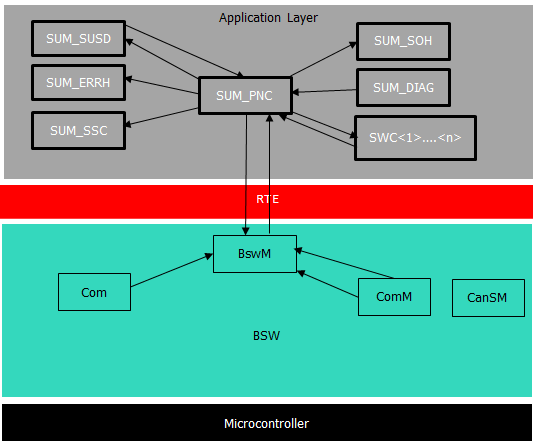
\includegraphics[scale=1.1]{images/layerDef.png}
\end{figure}

\noindent
For detailed information on it refer to Autosar.org website. Follows a short description of layers definition. 

\subsection{Application Layer}
Autosar Application layer consists of application software components, SUMs that are interdependent on each other for functional needs.
PNC interacts with other SUM modules in the application layer, the importance of interaction with those SUMs are explained briefly below:

\subsubsection{\textit{SUSD}}
SUSD provides signal to enable execution of PNC. Based on PN activity, PNC notifies this SUM for Shutdown permission.   

\subsubsection{\textit{SOH}}
Interface to publish PN$<$n$>$ failed attempt to start.

\subsubsection{\textit{SSC, ERRH, SOH}}
 Interfaces to publish Tx status notification (enabled/disabled).
 
\subsubsection{\textit{DIAG}}
DIAG Interface to PNC Provides notification to SUM\_PNC the status of diagnostics enabling or disabling of normal communications for each channel.

\subsubsection{\textit{SWC$<$1$>$...$<$n$>$}}
PNC interfaces to other SWCs to interface to Activation Criteria Signals:

\begin{itemize}
	\item $<$ActivationSensor\_n$>$ - signals that are read by a Sensor SW-C that is local to the ECU
	\item $<$ActivationSignal\_n$>$ - signals received via serial data communications that contribute to \textbf{local} activation criteria (\code{SUM\_PNC\_Criteria\_Signal\_Act}).
	\item $<$ActivationSignal\_Status\_n$>$ - signal status interface corresponding to each $<$ActivationSignal\_n$>$. Read inside \textit{Activation\_Signal\_In} together with the signal value; a signal only contributes to local activation when both its value and its status evaluate to TRUE.
	Note: Remote activation is driven exclusively by NM frames via the \textit{PNC\_NM\_Frame\_Indication} callback, not by these application signals.
	(These signals must be received via a different PN than the one which needs activation)
\end{itemize}

\subsection{RTE Layer}
Specifies the system function bus, main communication model etc.

\subsection{BSW Layer}
Provides BswM services via mode requester and mode user interfaces also services of communication stack are required by PNC.

\section{Generic Component Interface}
\label{section:GenericComponentIF}
Below table summarizes the interfaces associated with PNC and dependent/required modules.

%images
\begin{figure}[h!]
	\centering
	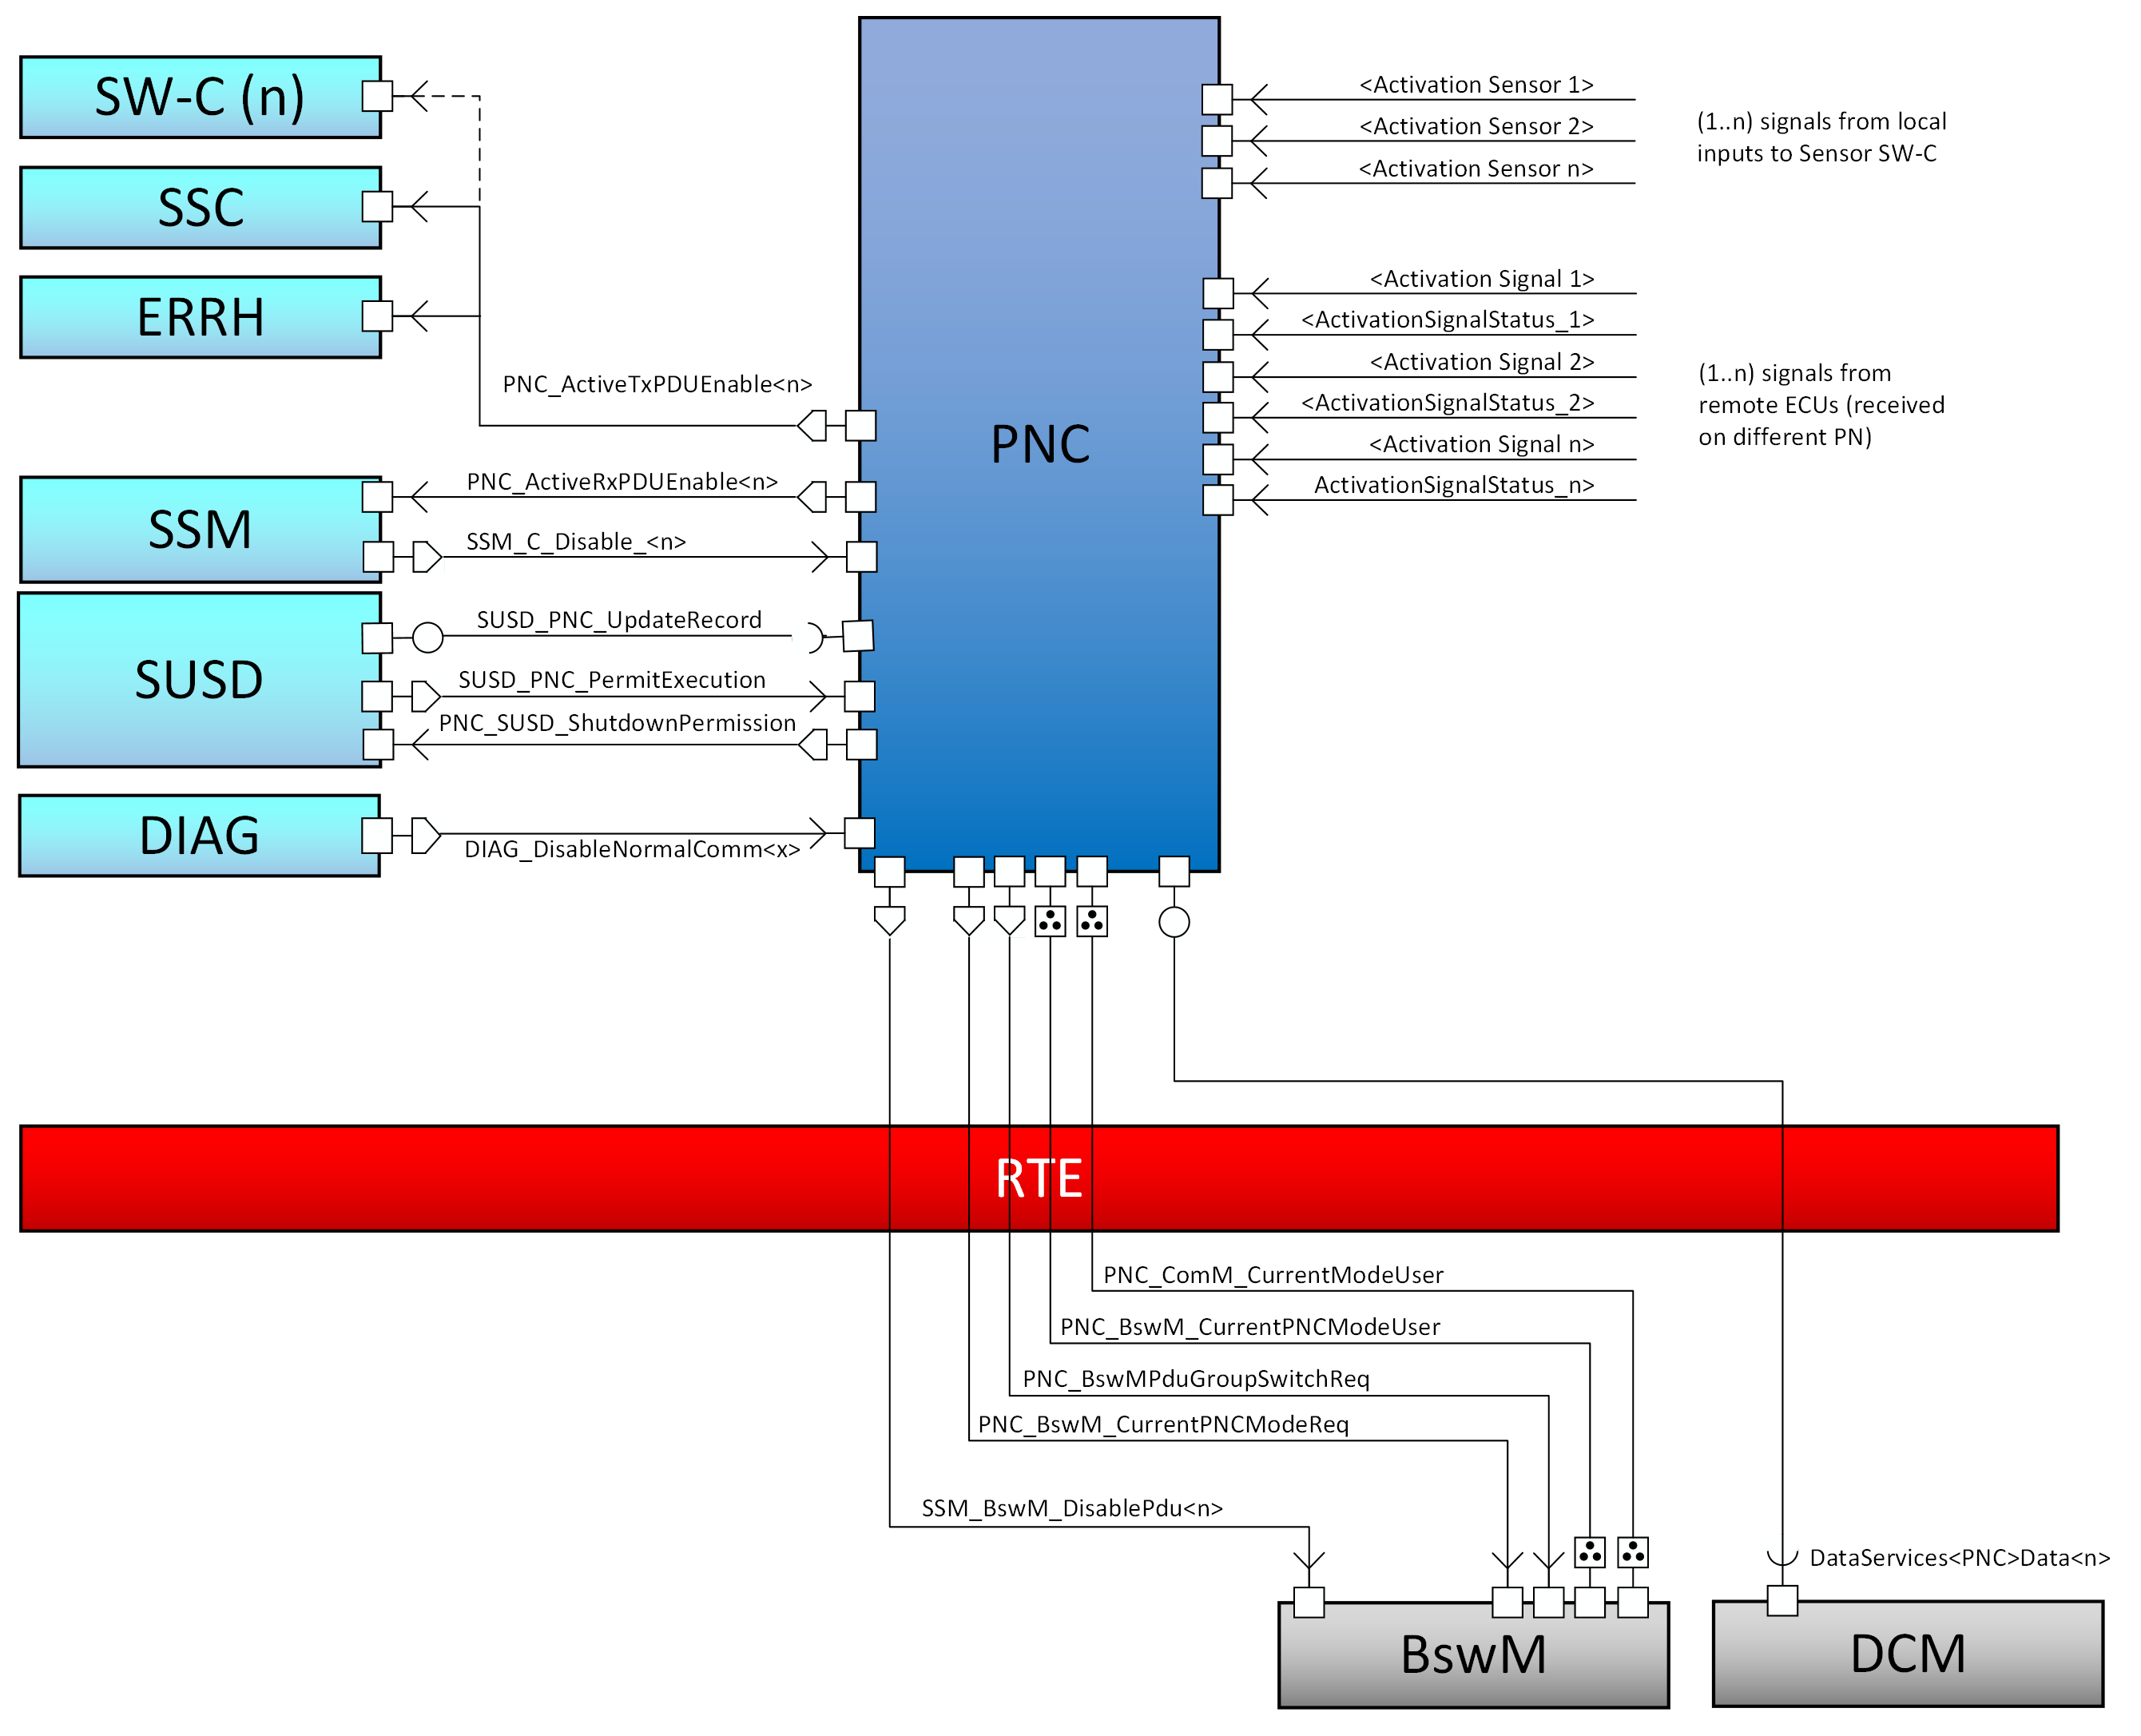
\includegraphics[scale=0.65]{images/blockDiagIF.png}
	\caption{SUM\_PNC Interfaces representation}
\end{figure}
\noindent
\noindent

\RequirementTag{SDD_PNC}{001}
\\
\begin{longtable}{|l|l|l|l|l|}
\hline
\begin{minipage}{0.33\linewidth}\raggedright\vspace{.75ex}{\cellcolor{eTASPurple}\textcolor{white}{\bfseries Port Interface} }\vspace{.75ex}\end{minipage} & \begin{minipage}{0.09\linewidth}\raggedright\vspace{.75ex}{\cellcolor{eTASPurple}\textcolor{white}{\bfseries  Port Type} }\vspace{.75ex}\end{minipage} & \begin{minipage}{0.09\linewidth}\raggedright\vspace{.75ex}{\cellcolor{eTASPurple}\textcolor{white}{\bfseries  P-Port} }\vspace{.75ex}\end{minipage} & \begin{minipage}{0.09\linewidth}\raggedright\vspace{.75ex}{\cellcolor{eTASPurple}\textcolor{white}{\bfseries  R-Port} }\vspace{.75ex}\end{minipage} & \begin{minipage}{0.24\linewidth}\raggedright\vspace{.75ex}{\cellcolor{eTASPurple}\textcolor{white}{\bfseries  Description} }\vspace{.75ex}\end{minipage}\\
\hline\hline
\endfirsthead
\hline
\begin{minipage}{0.33\linewidth}\raggedright\vspace{.75ex}{\cellcolor{eTASPurple}\textcolor{white}{\bfseries Port Interface} }\vspace{.75ex}\end{minipage} & \begin{minipage}{0.09\linewidth}\raggedright\vspace{.75ex}{\cellcolor{eTASPurple}\textcolor{white}{\bfseries  Port Type} }\vspace{.75ex}\end{minipage} & \begin{minipage}{0.09\linewidth}\raggedright\vspace{.75ex}{\cellcolor{eTASPurple}\textcolor{white}{\bfseries  P-Port} }\vspace{.75ex}\end{minipage} & \begin{minipage}{0.09\linewidth}\raggedright\vspace{.75ex}{\cellcolor{eTASPurple}\textcolor{white}{\bfseries  R-Port} }\vspace{.75ex}\end{minipage} & \begin{minipage}{0.24\linewidth}\raggedright\vspace{.75ex}{\cellcolor{eTASPurple}\textcolor{white}{\bfseries  Description} }\vspace{.75ex}\end{minipage}\\
\hline\hline
\endhead
\hline
\endfoot
\hline
\endlastfoot
\begin{minipage}{0.33\linewidth}\raggedright\vspace{.75ex}{\cellcolor{eTASGray30} \footnotesize{PNC\_ActiveTxPDUEnable<n>}}\vspace{.75ex}\end{minipage} & \begin{minipage}{0.09\linewidth}\raggedright\vspace{.75ex}{\cellcolor{eTASGray30}  \small{S/R}}\vspace{.75ex}\end{minipage} & \begin{minipage}{0.09\linewidth}\raggedright\vspace{.75ex}{\cellcolor{eTASGray30}  \small{SUM\_PNC}}\vspace{.75ex}\end{minipage} & \begin{minipage}{0.09\linewidth}\raggedright\vspace{.75ex}{\cellcolor{eTASGray30}  \small{SUM\_SSC, SUM\_ERRH and Local SW-Cs}}\vspace{.75ex}\end{minipage} & \begin{minipage}{0.24\linewidth}\raggedright\vspace{.75ex}{\cellcolor{eTASGray30}  \small{Notification that PN<n> is transmitting signals}}\vspace{.75ex}\end{minipage}\\\hline
\begin{minipage}{0.33\linewidth}\raggedright\vspace{.75ex}{\cellcolor{eTASGray30} \footnotesize{PNC\_ActiveRxPDUEnable<n>}}\vspace{.75ex}\end{minipage} & \begin{minipage}{0.09\linewidth}\raggedright\vspace{.75ex}{\cellcolor{eTASGray30}  \small{S/R}}\vspace{.75ex}\end{minipage} & \begin{minipage}{0.09\linewidth}\raggedright\vspace{.75ex}{\cellcolor{eTASGray30}  \small{SUM\_PNC}}\vspace{.75ex}\end{minipage} & \begin{minipage}{0.09\linewidth}\raggedright\vspace{.75ex}{\cellcolor{eTASGray30}  \small{SUM\_SSFM}}\vspace{.75ex}\end{minipage} & \begin{minipage}{0.24\linewidth}\raggedright\vspace{.75ex}{\cellcolor{eTASGray30}  \small{Notification to SSFM that PN<n> is receiving signals}}\vspace{.75ex}\end{minipage}\\\hline
\begin{minipage}{0.33\linewidth}\raggedright\vspace{.75ex}{\cellcolor{eTASGray30} \footnotesize{ShutdownPermission}}\vspace{.75ex}\end{minipage} & \begin{minipage}{0.09\linewidth}\raggedright\vspace{.75ex}{\cellcolor{eTASGray30}  \small{S/R}}\vspace{.75ex}\end{minipage} & \begin{minipage}{0.09\linewidth}\raggedright\vspace{.75ex}{\cellcolor{eTASGray30}  \small{SUM\_PNC}}\vspace{.75ex}\end{minipage} & \begin{minipage}{0.09\linewidth}\raggedright\vspace{.75ex}{\cellcolor{eTASGray30}  \small{SUM\_SUSD}}\vspace{.75ex}\end{minipage} & \begin{minipage}{0.24\linewidth}\raggedright\vspace{.75ex}{\cellcolor{eTASGray30}  \small{Notification to SUSD on activity/inactivity of PN}}\vspace{.75ex}\end{minipage}\\\hline
\begin{minipage}{0.33\linewidth}\raggedright\vspace{.75ex}{\cellcolor{eTASGray30} \footnotesize{PermitExecution}}\vspace{.75ex}\end{minipage} & \begin{minipage}{0.09\linewidth}\raggedright\vspace{.75ex}{\cellcolor{eTASGray30}  \small{S/R}}\vspace{.75ex}\end{minipage} & \begin{minipage}{0.09\linewidth}\raggedright\vspace{.75ex}{\cellcolor{eTASGray30}  \small{SUM\_SUSD}}\vspace{.75ex}\end{minipage} & \begin{minipage}{0.09\linewidth}\raggedright\vspace{.75ex}{\cellcolor{eTASGray30}  \small{SUM\_PNC}}\vspace{.75ex}\end{minipage} & \begin{minipage}{0.24\linewidth}\raggedright\vspace{.75ex}{\cellcolor{eTASGray30}  \small{Interface to provide signal to enable start/stop of PNC}}\vspace{.75ex}\end{minipage}\\\hline
\begin{minipage}{0.33\linewidth}\raggedright\vspace{.75ex}{\cellcolor{eTASGray30} \footnotesize{DIAG\_DisableNormalComm<channel>}}\vspace{.75ex}\end{minipage} & \begin{minipage}{0.09\linewidth}\raggedright\vspace{.75ex}{\cellcolor{eTASGray30}  \small{S/R}}\vspace{.75ex}\end{minipage} & \begin{minipage}{0.09\linewidth}\raggedright\vspace{.75ex}{\cellcolor{eTASGray30}  \small{SUM\_DIAG}}\vspace{.75ex}\end{minipage} & \begin{minipage}{0.09\linewidth}\raggedright\vspace{.75ex}{\cellcolor{eTASGray30}  \small{SUM\_PNC}}\vspace{.75ex}\end{minipage} & \begin{minipage}{0.24\linewidth}\raggedright\vspace{.75ex}{\cellcolor{eTASGray30}  \small{Provides notification to SUM\_PNC the status of diagnostics enabling or disabling of normal communications for each <channel>}}\vspace{.75ex}\end{minipage}\\\hline
\begin{minipage}{0.33\linewidth}\raggedright\vspace{.75ex}{\cellcolor{eTASGray30} \footnotesize{<ActivationSignal\_n>}}\vspace{.75ex}\end{minipage} & \begin{minipage}{0.09\linewidth}\raggedright\vspace{.75ex}{\cellcolor{eTASGray30}  \small{S/R}}\vspace{.75ex}\end{minipage} & \begin{minipage}{0.09\linewidth}\raggedright\vspace{.75ex}{\cellcolor{eTASGray30}  \small{SW-C (usually remote) or Dcm}}\vspace{.75ex}\end{minipage} & \begin{minipage}{0.09\linewidth}\raggedright\vspace{.75ex}{\cellcolor{eTASGray30}  \small{SUM\_PNC}}\vspace{.75ex}\end{minipage} & \begin{minipage}{0.24\linewidth}\raggedright\vspace{.75ex}{\cellcolor{eTASGray30}  \small{n interface(s) for every serial data signal or RID that is involved in a PNs activation and/or deactivation criteria.}}\vspace{.75ex}\end{minipage}\\\hline
\begin{minipage}{0.33\linewidth}\raggedright\vspace{.75ex}{\cellcolor{eTASGray30} \footnotesize{<ActivationSignal\_Status\_n>}}\vspace{.75ex}\end{minipage} & \begin{minipage}{0.09\linewidth}\raggedright\vspace{.75ex}{\cellcolor{eTASGray30}  \small{S/R }}\vspace{.75ex}\end{minipage} & \begin{minipage}{0.09\linewidth}\raggedright\vspace{.75ex}{\cellcolor{eTASGray30}  \small{SW-C (usually remote) or Dcm}}\vspace{.75ex}\end{minipage} & \begin{minipage}{0.09\linewidth}\raggedright\vspace{.75ex}{\cellcolor{eTASGray30}  \small{SUM\_PNC}}\vspace{.75ex}\end{minipage} & \begin{minipage}{0.24\linewidth}\raggedright\vspace{.75ex}{\cellcolor{eTASGray30}  \small{n interface(s) for every serial data signal or RID that is involved in a PNs activation and/or deactivation criteria}}\vspace{.75ex}\end{minipage}\\\hline
\begin{minipage}{0.33\linewidth}\raggedright\vspace{.75ex}{\cellcolor{eTASGray30} \footnotesize{<ActivationSensor\_n>}}\vspace{.75ex}\end{minipage} & \begin{minipage}{0.09\linewidth}\raggedright\vspace{.75ex}{\cellcolor{eTASGray30}  \small{C/S}}\vspace{.75ex}\end{minipage} & \begin{minipage}{0.09\linewidth}\raggedright\vspace{.75ex}{\cellcolor{eTASGray30}  \small{Sensor SW-C}}\vspace{.75ex}\end{minipage} & \begin{minipage}{0.09\linewidth}\raggedright\vspace{.75ex}{\cellcolor{eTASGray30}  \small{SUM\_PNC}}\vspace{.75ex}\end{minipage} & \begin{minipage}{0.24\linewidth}\raggedright\vspace{.75ex}{\cellcolor{eTASGray30}  \small{n C/S interface(s) to every sensor SW-C signal that is involved in a ECU's activation and/or deactivation criteria}}\vspace{.75ex}\end{minipage}\\\hline
\begin{minipage}{0.33\linewidth}\raggedright\vspace{.75ex}{\cellcolor{eTASGray30} \footnotesize{PNC\_BswM\_CurrentPNCModeUser<n>}}\vspace{.75ex}\end{minipage} & \begin{minipage}{0.09\linewidth}\raggedright\vspace{.75ex}{\cellcolor{eTASGray30}  \small{Mode User}}\vspace{.75ex}\end{minipage} & \begin{minipage}{0.09\linewidth}\raggedright\vspace{.75ex}{\cellcolor{eTASGray30}  \small{BswM}}\vspace{.75ex}\end{minipage} & \begin{minipage}{0.09\linewidth}\raggedright\vspace{.75ex}{\cellcolor{eTASGray30}  \small{SUM\_PNC}}\vspace{.75ex}\end{minipage} & \begin{minipage}{0.24\linewidth}\raggedright\vspace{.75ex}{\cellcolor{eTASGray30}  \small{Receives the status of PN<n> via BswM ComM\_CurrentPNCMode for n PN(s) in which the ECU participates}}\vspace{.75ex}\end{minipage}\\\hline
\begin{minipage}{0.33\linewidth}\raggedright\vspace{.75ex}{\cellcolor{eTASGray30} \footnotesize{PNC\_BswM\_CurrentPNCModeReq <n>}}\vspace{.75ex}\end{minipage} & \begin{minipage}{0.09\linewidth}\raggedright\vspace{.75ex}{\cellcolor{eTASGray30}  \small{Mode Request}}\vspace{.75ex}\end{minipage} & \begin{minipage}{0.09\linewidth}\raggedright\vspace{.75ex}{\cellcolor{eTASGray30}  \small{SUM\_PNC}}\vspace{.75ex}\end{minipage} & \begin{minipage}{0.09\linewidth}\raggedright\vspace{.75ex}{\cellcolor{eTASGray30}  \small{BswM}}\vspace{.75ex}\end{minipage} & \begin{minipage}{0.24\linewidth}\raggedright\vspace{.75ex}{\cellcolor{eTASGray30}  \small{Request activation / deactivation of PN<n>. For Activating ECU only.}}\vspace{.75ex}\end{minipage}\\\hline
\begin{minipage}{0.33\linewidth}\raggedright\vspace{.75ex}{\cellcolor{eTASGray30} \footnotesize{PNC\_ComM\_CurrentModeUser <n>}}\vspace{.75ex}\end{minipage} & \begin{minipage}{0.09\linewidth}\raggedright\vspace{.75ex}{\cellcolor{eTASGray30}  \small{Mode User}}\vspace{.75ex}\end{minipage} & \begin{minipage}{0.09\linewidth}\raggedright\vspace{.75ex}{\cellcolor{eTASGray30}  \small{BswM}}\vspace{.75ex}\end{minipage} & \begin{minipage}{0.09\linewidth}\raggedright\vspace{.75ex}{\cellcolor{eTASGray30}  \small{SUM\_PNC}}\vspace{.75ex}\end{minipage} & \begin{minipage}{0.24\linewidth}\raggedright\vspace{.75ex}{\cellcolor{eTASGray30}  \small{Receives the status of the communication channels<n> of the ECU via BswM\_ComMCurrentMode.}}\vspace{.75ex}\end{minipage}\\\hline
\begin{minipage}{0.33\linewidth}\raggedright\vspace{.75ex}{\cellcolor{eTASGray30} \footnotesize{PNC\_BswMPduGroupSwitchTxReq<n>}}\vspace{.75ex}\end{minipage} & \begin{minipage}{0.09\linewidth}\raggedright\vspace{.75ex}{\cellcolor{eTASGray30}  \small{Mode Request}}\vspace{.75ex}\end{minipage} & \begin{minipage}{0.09\linewidth}\raggedright\vspace{.75ex}{\cellcolor{eTASGray30}  \small{SUM\_PNC}}\vspace{.75ex}\end{minipage} & \begin{minipage}{0.09\linewidth}\raggedright\vspace{.75ex}{\cellcolor{eTASGray30}  \small{BswM}}\vspace{.75ex}\end{minipage} & \begin{minipage}{0.24\linewidth}\raggedright\vspace{.75ex}{\cellcolor{eTASGray30}  \small{Request start / stop of I-PDU Tx group <n>}}\vspace{.75ex}\end{minipage}\\\hline
\begin{minipage}{0.33\linewidth}\raggedright\vspace{.75ex}{\cellcolor{eTASGray30} \footnotesize{PNC\_BswMPduGroupSwitchRxReq<n>}}\vspace{.75ex}\end{minipage} & \begin{minipage}{0.09\linewidth}\raggedright\vspace{.75ex}{\cellcolor{eTASGray30}  \small{Mode Request}}\vspace{.75ex}\end{minipage} & \begin{minipage}{0.09\linewidth}\raggedright\vspace{.75ex}{\cellcolor{eTASGray30}  \small{SUM\_PNC}}\vspace{.75ex}\end{minipage} & \begin{minipage}{0.09\linewidth}\raggedright\vspace{.75ex}{\cellcolor{eTASGray30}  \small{BswM}}\vspace{.75ex}\end{minipage} & \begin{minipage}{0.24\linewidth}\raggedright\vspace{.75ex}{\cellcolor{eTASGray30}  \small{Request start / stop of I-PDU Rx group<n>}}\vspace{.75ex}\end{minipage}\\\hline
\begin{minipage}{0.33\linewidth}\raggedright\vspace{.75ex}{\cellcolor{eTASGray30} \footnotesize{DataServices\_PNC\_DID\_F08B\_Info\_Local}}\vspace{.75ex}\end{minipage} & \begin{minipage}{0.09\linewidth}\raggedright\vspace{.75ex}{\cellcolor{eTASGray30}  \small{S/R}}\vspace{.75ex}\end{minipage} & \begin{minipage}{0.09\linewidth}\raggedright\vspace{.75ex}{\cellcolor{eTASGray30}  \small{SUM\_PNC}}\vspace{.75ex}\end{minipage} & \begin{minipage}{0.09\linewidth}\raggedright\vspace{.75ex}{\cellcolor{eTASGray30}  \small{DCM}}\vspace{.75ex}\end{minipage} & \begin{minipage}{0.24\linewidth}\raggedright\vspace{.75ex}{\cellcolor{eTASGray30}  \small{Interface to DCM to get the local partial network activation status (Conditional, if it is allowed by ECU type)}}\vspace{.75ex}\end{minipage}\\\hline
\begin{minipage}{0.33\linewidth}\raggedright\vspace{.75ex}{\cellcolor{eTASGray30} \footnotesize{DataServices\_PNC\_DID\_F08D\_Info\_Remote}}\vspace{.75ex}\end{minipage} & \begin{minipage}{0.09\linewidth}\raggedright\vspace{.75ex}{\cellcolor{eTASGray30}  \small{S/R}}\vspace{.75ex}\end{minipage} & \begin{minipage}{0.09\linewidth}\raggedright\vspace{.75ex}{\cellcolor{eTASGray30}  \small{SUM\_PNC}}\vspace{.75ex}\end{minipage} & \begin{minipage}{0.09\linewidth}\raggedright\vspace{.75ex}{\cellcolor{eTASGray30}  \small{DCM}}\vspace{.75ex}\end{minipage} & \begin{minipage}{0.24\linewidth}\raggedright\vspace{.75ex}{\cellcolor{eTASGray30}  \small{Interface to DCM on remote partial activation status. (Conditional, if it is allowed by ECU type)}}\vspace{.75ex}\end{minipage}\\\hline
\begin{minipage}{0.33\linewidth}\raggedright\vspace{.75ex}{\cellcolor{eTASGray30} \footnotesize{PNC\_ComMPNC\_<n>\_Group\_DM\_Switch}}\vspace{.75ex}\end{minipage} & \begin{minipage}{0.09\linewidth}\raggedright\vspace{.75ex}{\cellcolor{eTASGray30}  \small{Mode Request}}\vspace{.75ex}\end{minipage} & \begin{minipage}{0.09\linewidth}\raggedright\vspace{.75ex}{\cellcolor{eTASGray30}  \small{SUM\_PNC}}\vspace{.75ex}\end{minipage} & \begin{minipage}{0.09\linewidth}\raggedright\vspace{.75ex}{\cellcolor{eTASGray30}  \small{BswM}}\vspace{.75ex}\end{minipage} & \begin{minipage}{0.24\linewidth}\raggedright\vspace{.75ex}{\cellcolor{eTASGray30}  \small{Request to enable or disable the deadline monitoring of the Rx PDU Group associated to PN<n>}}\vspace{.75ex}\end{minipage}\\\hline
\begin{minipage}{0.33\linewidth}\raggedright\vspace{.75ex}{\cellcolor{eTASGray30} \footnotesize{PN\_DTC\_Allowed\_<n>}}\vspace{.75ex}\end{minipage} & \begin{minipage}{0.09\linewidth}\raggedright\vspace{.75ex}{\cellcolor{eTASGray30}  \small{S/R}}\vspace{.75ex}\end{minipage} & \begin{minipage}{0.09\linewidth}\raggedright\vspace{.75ex}{\cellcolor{eTASGray30}  \small{SUM\_PNC}}\vspace{.75ex}\end{minipage} & \begin{minipage}{0.09\linewidth}\raggedright\vspace{.75ex}{\cellcolor{eTASGray30}  \small{SUM\_SSFM, SUM\_SSC}}\vspace{.75ex}\end{minipage} & \begin{minipage}{0.24\linewidth}\raggedright\vspace{.75ex}{\cellcolor{eTASGray30}  \small{Notification that a DTC against the PDUs of a specific PN can be set }}\vspace{.75ex}\end{minipage}\\\hline
\begin{minipage}{0.33\linewidth}\raggedright\vspace{.75ex}{\cellcolor{eTASGray30} \footnotesize{SUM\_C\_Disable\_<n>}}\vspace{.75ex}\end{minipage} & \begin{minipage}{0.09\linewidth}\raggedright\vspace{.75ex}{\cellcolor{eTASGray30}  \small{S/R}}\vspace{.75ex}\end{minipage} & \begin{minipage}{0.09\linewidth}\raggedright\vspace{.75ex}{\cellcolor{eTASGray30}  \small{SSFM}}\vspace{.75ex}\end{minipage} & \begin{minipage}{0.09\linewidth}\raggedright\vspace{.75ex}{\cellcolor{eTASGray30}  \small{PNC}}\vspace{.75ex}\end{minipage} & \begin{minipage}{0.24\linewidth}\raggedright\vspace{.75ex}{\cellcolor{eTASGray30}  \small{This interface is used to read the C\_Disable calibration provided by SSFM for Tx Pdu.}}\vspace{.75ex}\end{minipage}\\\hline
\begin{minipage}{0.33\linewidth}\raggedright\vspace{.75ex}{\cellcolor{eTASGray30} \footnotesize{SUM\_BswM\_DisablePdu<n>}}\vspace{.75ex}\end{minipage} & \begin{minipage}{0.09\linewidth}\raggedright\vspace{.75ex}{\cellcolor{eTASGray30}  \small{S/R}}\vspace{.75ex}\end{minipage} & \begin{minipage}{0.09\linewidth}\raggedright\vspace{.75ex}{\cellcolor{eTASGray30}  \small{PNC}}\vspace{.75ex}\end{minipage} & \begin{minipage}{0.09\linewidth}\raggedright\vspace{.75ex}{\cellcolor{eTASGray30}  \small{BswM}}\vspace{.75ex}\end{minipage} & \begin{minipage}{0.24\linewidth}\raggedright\vspace{.75ex}{\cellcolor{eTASGray30}  \small{Mode interface with the BswM to disable the Pdu with PduID.}}\vspace{.75ex}\end{minipage}\\\hline
\end{longtable}

\Satisfies{SRS\_PNC 008} \Satisfies{SRS_PNC 002} \Satisfies{SRS_PNC 048}  \Satisfies{SRS_PNC 049} \Satisfies{SRS_PNC 050} \Satisfies{SRS_PNC 051}     \Satisfies{SRS_PNC 052} \Satisfies{SRS_PNC 053} \Satisfies{SRS_PNC 013} \Satisfies{SRS_PNC 020} \Satisfies{SRS_PNC 023} \Satisfies{SRS_PNC 026}

\textbf{NOTE:}

\begin{enumerate}
	\item The notation used for Naming the module: \textit{SUM\_$<$name of the module$>$}
	\item SUM\_PNC for Partial Network Coordinator;
	\item This notation is used for naming interfaces: \textit{$<$SUM Module Name$>$\_$<$Interacting Module Name$>$\_$<$Interface Name$>$}
	\begin{itemize}
		\item Example: \textit{PNC\_BswM\_CurrentPNCModeUser$<$n$>$}
	\end{itemize}
	\item This notation is used for representing states:\newline [\$Satisfies \$SRS\_$<$SUM Module Name$>$ $<$requirement ID$>$]
	\item This notation is used for specific APIs, where interactions are involved with BswM module:
	[RTE\_callSpecificSuffix]\_[RTE\_Port\_Name\_$<$PartialNetworkID$>$\_$<$ComMChannelID$>$\_$<$PNCUserID$>$]\_[VDP]]. Example:
	\begin{enumerate}[label=\Alph*.]
		\item Rte\_Mode\_RP\_BswM\_ComM\_Current\_PNC\_ModeUser0\_6\_5\_PNC\_State
		\item Rte\_Write\_PP\_PNC\_BswM\_ComM\_CurrentPNCMode\_Req0\_6\_5\_PNC\_State
	\end{enumerate}
\end{enumerate}

\section{Assumptions and constraints}

\begin{itemize}
	\item All through the PN state machine, the condition check with naming convention \textbf{PN\_Activation\_Criteria$<$n$>$} is assumed to be a check for Local Activation and is maintained in that way all through the code;
	\item The user/integrator should ensure that the ComM Channels referred in "ComM\_PNC\_Ref" of Partial Network configuration under \textbf{PNC/PNCConfigSets/SUM\_PNC\_PARTIAL\_NETWORK\_PARAMETERs} should match with ComM channels configured in "ComM\_Channel\_Ref" under \textbf{PNC/PNCGeneral/ComM\_PNC\_Channels}.  
\end{itemize}

\subsubsection{Design Decision}

\begin{itemize}
	\item All the Port interfaces will have ComMPnc ShortName (assumed to be following PN names specified in [R2]) appended in the end, e.g.:\\
	The RPort \textit{RP\_Bswm\_ComM\_Current\_PNC\_ModeUser\_Propulsion} and the associated interface \textit{PNC\_BswM\_ComM\_CurrentPNCModeUser\_Propulsion} are created for Propulsion Partial Network.
\end{itemize}
